\documentclass[11pt]{article}
\usepackage[a4paper,top=3cm,bottom=3cm,left=2.5cm,right=2.5cm]{geometry}
\usepackage[italian]{babel}
\usepackage[utf8x]{inputenc}
\usepackage {caption}
\usepackage {url}
\usepackage {multirow}
\usepackage {booktabs}
\usepackage {fixltx2e}
\usepackage {float}
\usepackage {graphicx}
\usepackage {cite}
\usepackage {listings}
\usepackage {color}
\usepackage {xcolor,colortbl}
\usepackage {adjustbox}
\usepackage {array}
\usepackage {svg}
\usepackage {subfig}
\usepackage {amssymb}
\usepackage {hyperref}
\usepackage {tabulary}
\usepackage {tabularx}
\usepackage[T1]{fontenc}
\usepackage{wasysym}
\usepackage{enumitem}
\usepackage{lipsum}

\newcommand{\voceU}[1]{%
	\item #1\dotfill\Square%
}

\newcommand{\voceD}[1]{%
	\item #1\hfill\Square%
}
\hypersetup{colorlinks=true,citecolor=black,linkcolor=black, urlcolor=blue}

\date{}

\renewcommand{\lstlistingname}{Listato}


\lstset{
    language=C,
    basicstyle=\ttfamily,
    breaklines=true,
    frame=single, % draw a frame at the top and bottom of the code block
    tabsize=2, % tab space width
    showstringspaces=false, % don't mark spaces in strings
    numbers=left, % display line numbers on the left
    captionpos=b,
    commentstyle=\color{green}, % comment color
    keywordstyle=\color{blue}, % keyword color
    stringstyle=\color{red} % string color
}

\begin{document}

\title{\textbf{Definizione ed Implementazione di un Sistema di Raccomandazione Distribuito per film
		e Modellazione di Eventi Complessi}}

\author{\\\textit{Prof. Ing.} Tommaso di Noia\\\textit{Prof.ssa} Marina Mongiello \\
	Mauro Losciale\\ 
	Pietro Tedeschi\\}

\clearpage\maketitle
\thispagestyle{empty}

\begin{center}
	
\includegraphics[scale=0.40]{images/poliba.jpg}
\end{center}

{\textbf{\center Logica e Intelligenza Artificiale\\Ingegneria del Software Avanzata\\ Laurea Magistrale in Ingegneria Informatica\\Politecnico di Bari\\A.A 2015 - 2016\\}}

\newpage
\clearpage
\thispagestyle{empty}
\renewcommand\contentsname{Indice}
\tableofcontents
\newpage
\setcounter{page}{1}

\newpage
\section{Introduzione}
\section{Stato dell'arte}

\subsection{Introduzione ai sistemi CEP}
L'incremento dei dispositivi interconnessi e delle applicazioni distribuite, richiede un'elaborazione continua del flusso dati. Esempi di tali applicazioni, vanno dal traffico generato dalle Wireless Sensor Networks (WSN) al flusso dati relativo agli indici finanziari, dal monitoraggio stradale alla Clickstream Analysis. 

Un sistema ad eventi complessi, meglio conosciuto come \textit{Complex Event Processing} (CEP), modella il flusso informativo dei dati, visualizzando gli elementi come notifiche di ciò che sta accadendo nel mondo esterno. I dati vengono rilevati e filtrati utilizzando dei pattern (oppure le \textit{processing rules}), i quali hanno il compito di rappresentare il modello di riferimento con l'informazione da rilevare, per poi farla pervenire alle rispettive parti (ad esempio, i dispositivi che effettuano una sottoscrizione ad un determinato topic nel paradigma \textit{publish-subscribe}). L'obiettivo di un sistema CEP consiste nell'identificare eventi significanti e rispondere ad essi nel più breve tempo possibile.
Un pattern o una regola, può essere definita mediante un linguaggio basato su query, il cosiddetto \textbf{Event Query
	Language}.
\begin{figure}[H]
	\centering
	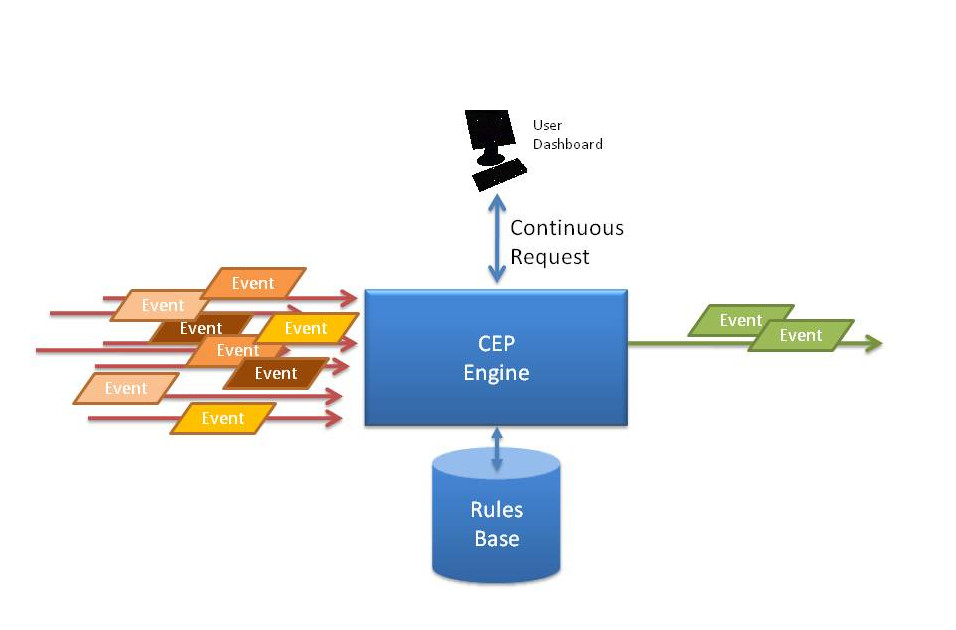
\includegraphics[scale=0.50]{images/CEP2.jpg}
	\caption{Architettura di un Sistema CEP\cite{cepimage}}
	\label{archcep}
\end{figure}

Gli \textbf{Event Query Languages} possono essere raggruppati in tre categorie: Composition Operators, Data Stream Query Languages e
Production Rules. I Composition Operators identificano gli eventi complessi partendo dalla composizione dei singoli eventi, utilizzando operatori quali congiunzione, negazione o di sequenza per la costruzione delle espressioni. Esempi rilevanti sono IBM Active Middleware Technology e ruleCore. 

I \textbf{Data Stream Query Languages} sono basati sul linguaggio SQL; gli stream di dati sono semplicemente tuple convertite per database relazionali, in modo che si possano eseguire query SQL su di esse. E' utile citare i seguenti approcci: CQL, Coral8, StreamBase,
Aleri, Esper e così via.

Le \textbf{Production Rules} specificano le azioni che devono essere eseguite quando il sistema si trova in determinati stati; non è un linguaggio ad eventi, ma costituisce un approccio importante nei sistemi CEP. Un esempio pratico è TIBCO Business Events.

Un altro fattore importante è il tempo. Sono due le parti da considerare quando si parla del tempo, il tempo della finestra ed il tempo dell'evento informativo. Il tempo della finestra mostra gli eventi che vengono esaminati in un determinato intervallo. Il tempo dell'evento invece, porta con se informazioni relative alla data, ora di rilevazione, tempo di transizione, ed intervallo di elaborazione.

I contributi relativi ai sistemi CEP, arrivano da diverse comunità, a partire da quelle che si occupano di sistemi distribuiti, automazione industriale, sistemi di controllo, monitoraggio delle reti, Internet of Things, e middleware in generale.

\begin{figure}[H]
	\centering
	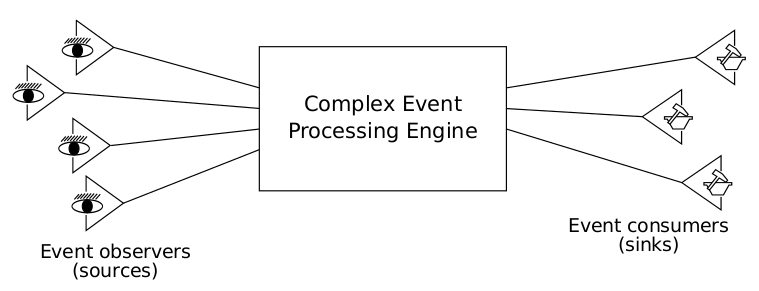
\includegraphics[scale=0.40]{images/CEP.png}
	\caption{Funzionamento di un Sistema CEP (High-Level) \cite{Cugola:2012:PFI:2187671.2187677}}
	\label{funcep}
\end{figure}

Come possiamo vedere dalla Figura \ref{funcep}, viene associata una semantica dettagliata agli elementi informativi da processare. Da una parte abbiamo gli \textbf{Event Observer}, i quali rappresentano la sorgente dei dati e degli eventi da notificare; in seguito abbiamo il \textbf{CEP Engine}, responsabile del filtraggio e della notifica degli eventi ai nodi \textit{sink}, identificati come \textbf{Event Consumers} \cite{Cugola:2012:PFI:2187671.2187677,fulop2010survey}.

\subsection{Sistemi di Raccomandazione}
\subsubsection{Filtro collaborativo}
\subsection{Introduzione allo Stream Processing}
\subsubsection{Il paradigma Publish-Subscribe}
\subsection{Il pattern Facade}
\subsection{Il pattern Singleton}
\subsection{Il pattern Model-View-Controller (MVC)}
\subsection{La tecnologia WebSocket}

\section{Analisi del progetto}

\section{Soluzione proposta}

\subsection{La libreria Spark}

Apache Spark è un sistema di cluster computing di tipo general-purpose, scalabile e veloce. Dispone di API di alto livello in \textbf{Java}, \textbf{Scala},\textbf{ Python} ed \textbf{R}, e un engine ottimizzato che supporta grafi di esecuzione generici. Integra inoltre un ampio set di tool come \textbf{Spark SQL}, per structured data processing, \textbf{MLlib} per il machine learning e \textbf{Spark Streaming}, descritti nelle sezioni successive. Spark è eseguibile sia su sistemi Windows che UNIX-like (Linux, Mac OS) \cite{spark}. \\

Una delle possibili configurazioni di un sistema Spark è la modalità \textit{cluster}, mostrata in Figura \ref{spark-cluster}. 

\begin{figure}[H]
	\centering
	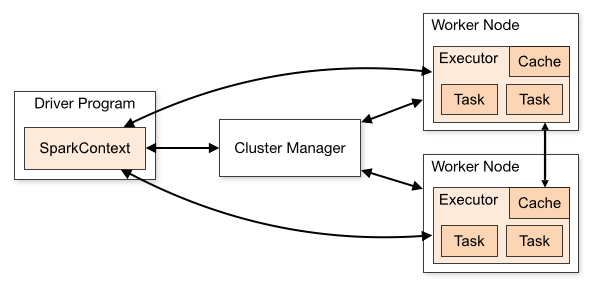
\includegraphics[scale=0.50]{images/cluster-overview.png}
	\caption{Configurazione in Spark di tipo Cluster Mode \cite{spark}}
	\label{spark-cluster}
\end{figure}

Le applicazioni Spark sono eseguite come un set di processi indipendenti sul cluster, coordinati dall'oggetto \textit{SparkContext} del programma sorgente (detto \textbf{driver program}). Precisamente, il programma driver può connettersi su diversi tipi di \textit{cluster managers} (ad esempio un cluster di tipo Standalone, Mesos o YARN), il quale alloca le risorse a disposizione delle applicazioni. Una volta connesso, Spark scansiona i nodi del cluster alla ricerca degli \textbf{executor} (detti anche \textit{worker node}), i quali eseguono effettivamente i task e il data storage delle applicazioni. A questo punto il driver invia il codice dell'applicazione agli executor (tipicamente un file JAR o Python incluso nello SparkContext) e schedula i task per l'esecuzione parallela \cite{spark}. 

Alcune considerazioni riguardo tale architettura sono: 
\begin{itemize}
	\item Ogni applicazione gestisce i propri workers, i quali restano attivi durante tutto il ciclo di vita ed eseguono task multipli in thread multipli. Questo implica un isolamento tra le applicazioni, sia lato scheduling (ogni driver schedula i propri tasks) sia lato executor (tasks relativi ad applicazioni differenti risiedono in JVM differenti). Tuttavia ciò implica che non è possibile condividere nativamente i dati tra applicazioni diverse, a meno di utilizzare uno storage system esterno;
	\item Il driver deve poter gestire le connessioni con i workers durante l'intero ciclo di vita dell'applicazione. Per questo motivo dev'essere sempre garantita la visibilità a livello di rete tra driver e workers durante l'esecuzione;
	\item \`E necessario che driver e worker abbiano, a livello di rete, una distanza relativamente breve, preferibilmente nella stessa LAN, affinché lo scheduling sia rapidamente eseguito \cite{spark}. 
\end{itemize}

Il principio di funzionamento di Spark si basa sostanzialmente sul concetto di \textit{Resilient Distributed Dataset} (\textbf{RDD}). Un RDD è una collezione di dati su cui è possibile operare parallelamente, ed è distribuita su tutti i nodi del cluster come file system Hadoop oppure è generata da una collezione esistente in Java o Scala \cite{spark}. \\

Una seconda astrazione è rappresentata dalle variabili condivise (\textit{shared variables}), utilizzate nelle computazioni parallele. Di default Spark tiene traccia delle variabili istanziate nei vari task, e consente se necessario di condividerle fra task o fra task e driver. Le variabili condivise possono essere di due tipi: di tipo \textit{broadcast}, il cui valore viene salvato nella cache per ogni nodo, e di tipo \textit{accumulatore}, per esempio contatori o sommatori \cite{spark}.

\subsubsection{Spark Streaming}

Spark Streaming è un'estensione delle Core API di Spark per lo\textbf{ stream processing} di live data streams ad alto throughput. Supporta molteplici sorgenti di data stream come\textbf{ Kafka}, Flume, Twitter, ZeroMQ, Kinesis o socket TCP, i quali possono essere processati tramite direttive come \textit{map}, \textit{join}, \textit{reduce} e \textit{window}. Nel post processing è possibile salvare i data stream in un file system, in un database o visualizzarli in una live dashboard. Come ulteriore fase nella pipeline di operazione rientra anche il machine learning ed il graph processing. In Figura \ref{spark-streaming} viene riassunta l'architettura descritta \cite{spark}. 

\begin{figure}[H]
	\centering
	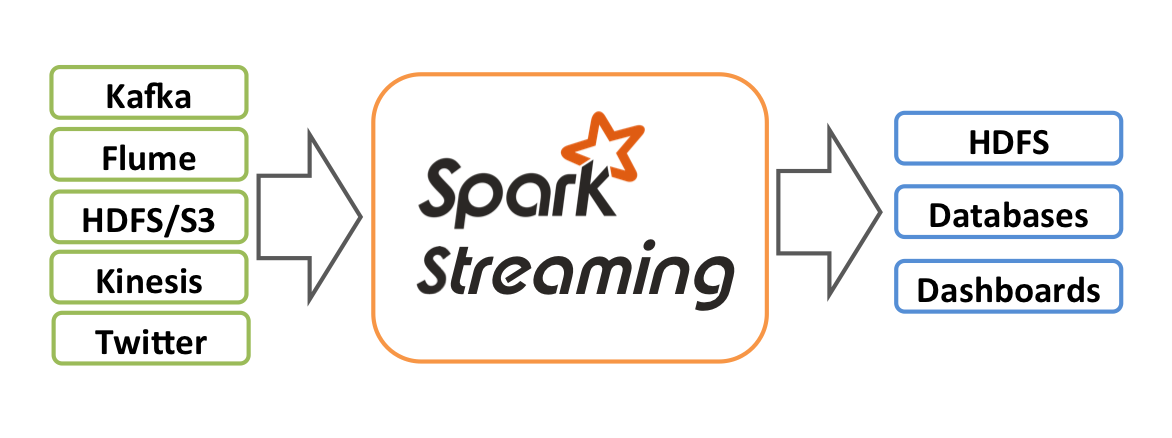
\includegraphics[scale=0.50]{images/streaming-arch.png}
	\caption{Architettura di Spark Streaming \cite{spark}}
	\label{spark-streaming}
\end{figure}

Nello specifico, i data streams ricevuti vengono suddivisi in frammenti (\textit{batches}), processati da Spark per generare lo stream finale risultante in batches, come mostrato in Figura \ref{spark-streaming-processing} \cite{spark}.

\begin{figure}[H]
	\centering
	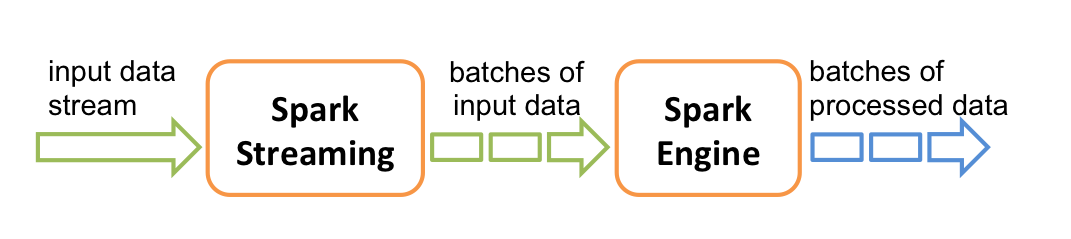
\includegraphics[scale=0.50]{images/streaming-flow.png}
	\caption{Spark Streaming Data Stream Processing \cite{spark}}
	\label{spark-streaming-processing}
\end{figure}

A livello alto il flusso continuo di dati è rappresento da una struttura astratta detta \textit{discretized stream} o \textit{DStream}, il cui contenuto è rappresentato da tutte le sorgenti collegate eventualmente con Spark, o da stream risultati da altri DStream. Internamente, un DStream è rappresentato tramite una sequenza di RDD \cite{spark}. 

\subsubsection{Spark MLlib}

Spark MLlib è la libreria per il machine learning di Spark, ed il suo obiettivo è di rendere l'uso di tali funzionalità semplice e scalabile. Comprende i più comuni algoritmi di learning quali classificazione, regressione, clustering, filtro collaborativo, riduzione dello spazio delle features, etc. \cite{spark}. 

\subsubsection{Spark SQL}

Spark SQL è un modulo di Spark per il processing di dati strutturati. A differenza delle API RDD la sua interfaccia consente di descrivere in maniera dettagliata la struttura e le operazioni da eseguire sui dati, in stile SQL. Le strutture astratte di riferimento per questo modulo sono i \textbf{Dataframes} e i \textbf{Datasets} \cite{spark}.\\

Un \textbf{Dataframe} è un collezione distribuita di informazioni organizzata in colonne e attributi. Concettualmente è equivalente ad una tabella in un database relazionale, con caratteristiche aggiuntive fornite da Spark. In accordo con tale definizione sono presenti, oltre alle classiche funzionalità SQL, la creazione di DataFrame a partire da un RDD o un oggetto JSON e viceversa \cite{spark}.\\

Un \textbf{Dataset} invece è un'interfaccia sperimentale introdotta nella versione 1.6 di Spark, mirata all'integrazione delle API RDD con l'engine SQL. Attualmente il supporto è limitato alle API Java e Scala \cite{spark}.

\subsection{Apache Kafka}

Apache Kafka è un sistema di messaggistica di tipo publish-subscribe, orientato alla distribuzione. La sua architettura consente ad un singolo cluster di agire da backbone centrale per i dati di grandi organizzazioni, e gli stream vengono partizionati e distribuiti lungo tutti i nodi del cluster, sfruttando la potenza di calcolo di ogni singola macchina. Di seguito si introduce la terminologia utilizzata in Kafka: 

\begin{itemize}
	\item Kafka organizza i flussi dei messaggi in categorie chiamate \textit{topics};
	\item I processi che si occupano di pubblicare i messaggi in Kafka sono chiamati \textit{producers};
	\item I processi che effettuano una sottoscrizione ad un topic ed elaborano i messaggi pubblicati sullo stesso sono chiamati \textit{consumers};
	\item I nodi all'interno del cluster(producers e consumers) sono coordinati da uno o più server chiamati \textit{brokers} \cite{kafka}.
	
\end{itemize}

A livello concettuale il funzionamento di Kafka è riassunto in Figura \ref{kafka}. La comunicazione tra client e server avviene tramite protocollo TCP. Sono presenti varie implementazioni del client Kafka, disponibili in vari linguaggi tra cui Java, Javascript e PHP \cite{kafka}. 

\begin{figure}[H]
	\centering
	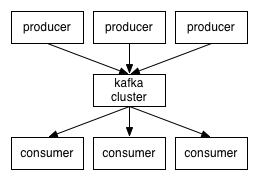
\includegraphics[scale=0.80]{images/kafka.png}
	\caption{Architettura di Apache Kafka \cite{kafka}}
	\label{kafka}
\end{figure}


Di seguito viene mostrata nel dettaglio la struttura di un topic in Figura \ref{kafka-topic}. Per ogni topic Kafka effettua un partizionamento dei messaggi in arrivo, tenendo traccia dell'ordine di arrivo con un sistema di log \cite{kafka}. 

\begin{figure}[H]
	\centering
	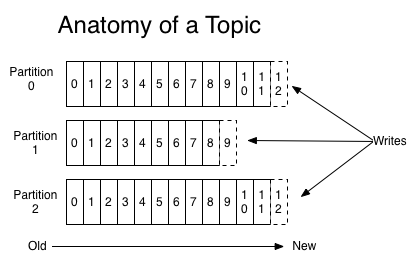
\includegraphics[scale=0.80]{images/log_anatomy.png}
	\caption{Struttura di un topic in Kafka \cite{kafka}}
	\label{kafka-topic}
\end{figure}

Ogni partizione è una sequenza immutabile di messaggi, registrata e ordinata in un commit log. Ad ogni messaggio presente viene assegnato un id sequenziale, detto \textit{offset}, che identifica univocamente un messaggio nella relativa partizione \cite{kafka}.

Il cluster di Kafka conserva in memoria tutti i messaggi pubblicati, letti o non dai consumers, per un periodo di tempo configurabile. In pratica, il server registra dei metadati relativi ad ogni posizione del consumer nel log, chiamato appunto offset. Tale offset è fissato dal consumer, il quale può leggere i messaggi nell'ordine preferito \cite{kafka}. 


\subsubsection{Integrazione con Spark Streaming}

\subsection{Il framework Node.js}
\subsubsection{Panoramica}
\subsubsection{Kafka Client per Node.js}
\subsubsection{Il framework Angular.js}
\subsection{La libreria socket.IO}

\section{Conclusioni e sviluppi futuri}

\clearpage
\addcontentsline{toc}{section}{Bibliografia}
\nocite{*}
\bibliographystyle{plain}
\bibliography{biblib}


\end{document}